\chapter{Introduction and Literature Review}

This chapter contains my introduction and literature review. We might define
$m$\nomenclature{$m$}{Mass} as the mass of some object. We might also cite a
book as~\cite{lacava1992}. See Figure~\ref{fig:panel-al4} or
Table~\ref{table:amplitude} for more information.
\begin{figure}[tbp]
\centering
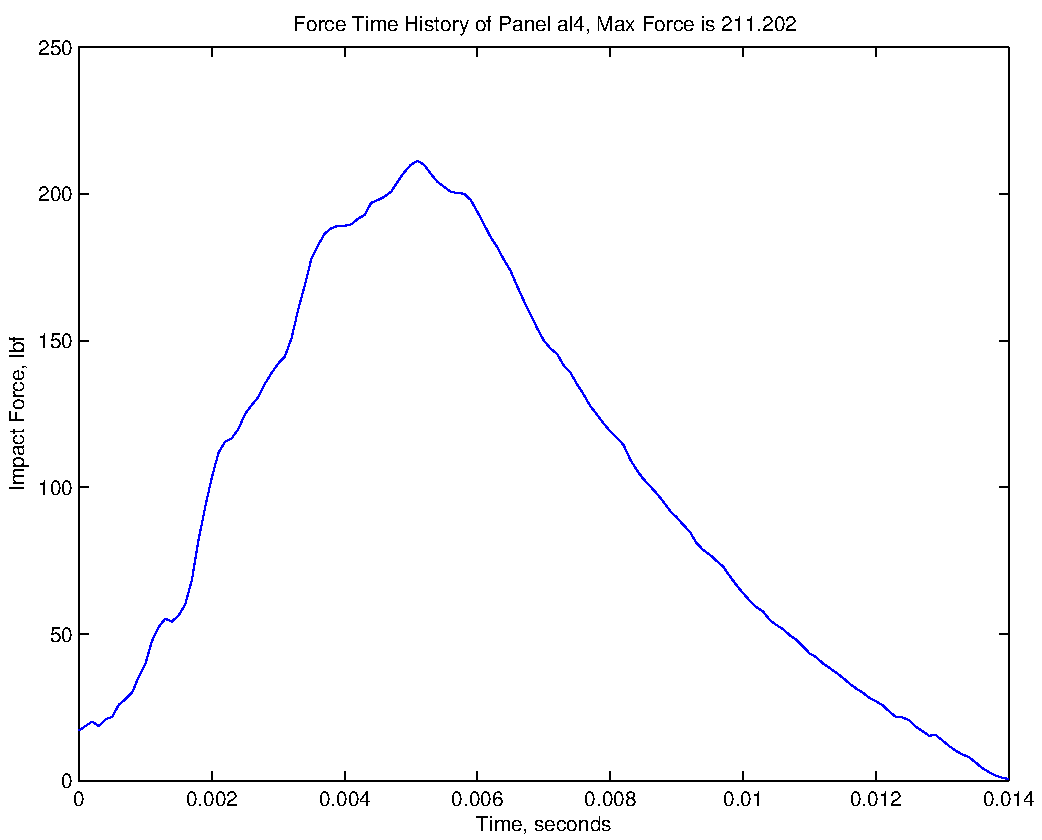
\includegraphics[width=\textwidth]{al4-1}
\caption{Force Time History of Panel ``al-4''\label{fig:panel-al4}}
\end{figure}
\begin{table}
\caption{GNU Radio Amplitude and Corresponding Voltages\label{table:amplitude}}
\centering
% \begin{tabular}{SSS}
% \toprule
% % text headers often need to be enclosed in braces to keep siunitx from
% % mis-interpreting them as units
% {GNU Radio Amplitude} & {Oscilloscope} & {Calculated Power} \\ 
%  & \si{\mvrms} & \si{\dbm} \\
% \midrule
% 0.1 &  28.5 & -8.946 \\
% 0.2 &  57.1 & -5.928 \\
% 0.3 &  85.2 & -4.190 \\
% 0.4 & 116.5 & -2.831 \\
% 0.5 & 140.4 & -2.021 \\
% 0.6 & 167.5 & -1.255 \\
% 0.7 & 196.9 & -0.552 \\
% 0.8 & 227.3 &  0.071 \\
% 0.9 & 257.2 &  0.608 \\
% 1.0 & 273.9 &  0.881 \\
% 1.5 & 273.6 &  0.876 \\tokentoken
% 2.0 & 273.6 &  0.876 \\
% 2.5 & 273.4 &  0.873 \\
% 3.0 & 274.1 &  0.884 \\
% 3.5 & 273.2 &  0.870 \\
% 4.0 & 269.7 &  0.814 \\
% 4.5 & 271.6 &  0.845 \\
% 5.0 & 273.7 &  0.878 \\
% \bottomrule
% \end{tabular}
\end{table}